\documentclass[letterpaper, 12pt]{article}
\usepackage{graphicx}
\usepackage{titling}
\usepackage{float}
\usepackage{csvsimple}

\title{RLC Series Circuit}
\date{December 7, 2019}
\author{Faris Hijazi\\
        Phys 4B 1:00-3:50\\}
\begin{document}
\begin{titlingpage}
    \maketitle
    \begin{abstract}
        An RLC circuit is an electrical circuit with a resistor, inductor or capacitor 
 connected in series or parallel but in this lab, they are connected in series.
 RLC circuits form harmonic oscillators with a peak resonant frequency. The purpose of the 
 lab was to experimentally measure the resonant frequency of an RLC circuit (175Hz) and 
 compare it to the theoretical resonant frequency (175.75Hz). The resulting percent difference
 was 0.42\%.
    \end{abstract}
\end{titlingpage}


\section*{Introduction} 
The purpose of this lab was to experimentally measure 
the resonant frequency of an RLC circuit by recording peak voltages
in an RLC circuit generated by a frequency generator.
Comparing the experimental frequency to the theoretical resonant 
frequency is done to verify that RLC circits have a resonant frequency which is 
$f_{resonant} = \frac{1}{2 \pi \sqrt{L C}}$. 


\section*{Equipment}

\begin{itemize}
    \item RLC circuit board
    \item digital multimeter
    \item function generator
    \item function generator powersupply
    \item wire leads
\end{itemize}

\begin{figure}[H]
    \centering
    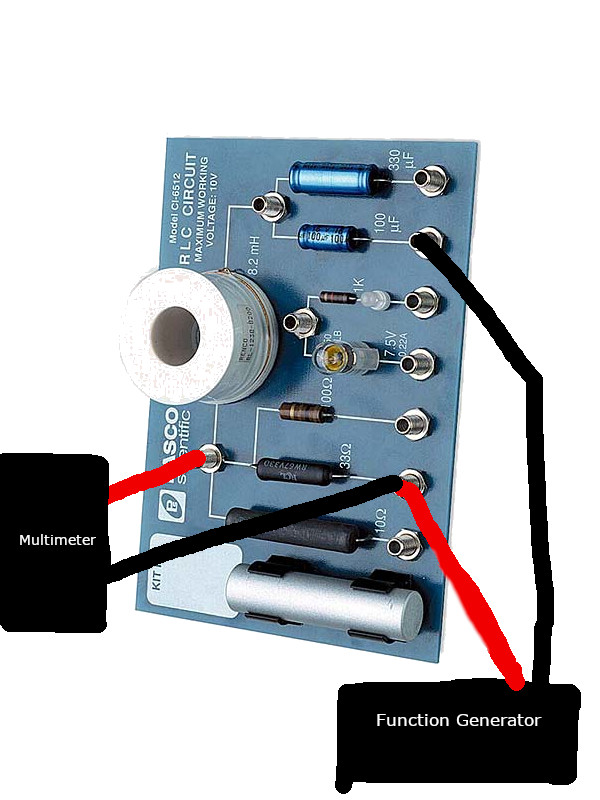
\includegraphics[height=4.6in]{rlc circuit}
    \caption{apparatus}
    \label{fig: rlc circuit}
\end{figure}

\section*{Theory}

\begin{table}[H]
\begin{tabular}{|l|l|}
\hline
\textbf{Variable} & \textbf{Definition} \\
    \hline
    $X_c$ & capacitive reactance \\
    \hline
    $X_l$ & inductive reactance \\
    \hline
    $L$ & inductance \\
    \hline
    $C$ & capacitance \\
    \hline
    $f$ & frequency \\
    \hline
    $f_{resonant}$ & resonant frequency \\
    \hline
\end{tabular}
\end{table}

\begin{center}

$X_c = \frac{1}{2 \pi f C}$

$X_l = 2 \pi f L$
\linebreak

f is resonant when $X_c = X_l$

\begin{equation}
    f^2 = \frac{1}{4 \pi^2 L C}
\end{equation}
\begin{equation}
    f_{resonant} = \frac{1}{2 \pi \sqrt{L C}}
\end{equation}
\begin{equation}
    \frac{|Theoretical - Experimental|}{Theoretical}100 = Percent Difference
\end{equation}
\end{center}



\section*{Procedure}

\begin{enumerate}
    \item Set frequency of the function generator to 60hz, 
    then, adjust the output voltage to 5V (measured on voltmeter)
    \item Connect leads to circuit as shown in Figure \ref{fig: rlc circuit}
    \item measure peak voltage across the resistor for a variety of frequencies
    ranging from 10-500000hz
    \item create a graph of voltage vs frequency to determine the experimental 
    resonant frequency 
\end{enumerate}

\section*{Analysis}
\begin{center}
    Theoretical Resonant frequency: $f_{resonant} = \frac{1}{2 \pi \sqrt{8.2mH * 100 \mu f }}$

    $f_{theory} = 175.75hz$

    Experimental Resonant frequency: $\frac{150+200}{2}$

    $f_{exp} = 175hz$

    Percent Difference: $\frac{|175.75 - 175|}{175.75}100 = 0.42\%$
\end{center}
\subsection*{Data}

\begin{figure}[H]
    \csvautotabular{test.csv}
    \label{fig: data}
\end{figure}

\begin{figure}[H]
    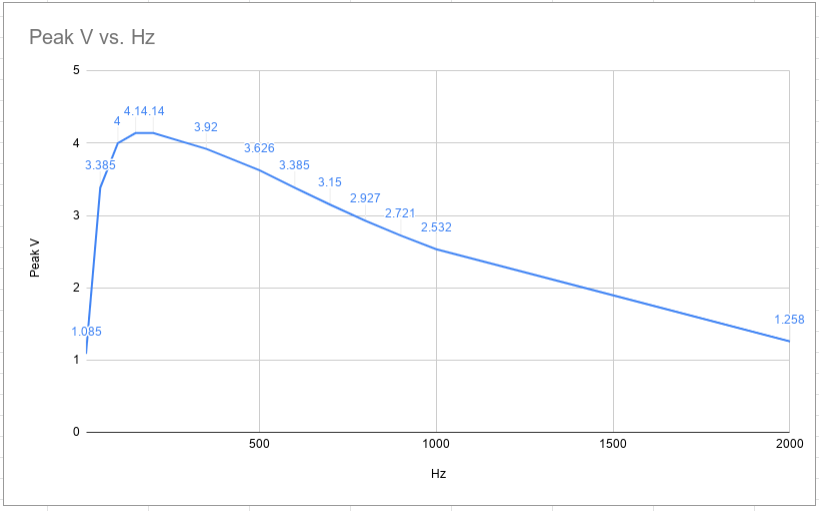
\includegraphics[width=\textwidth]{graph1}
    \caption{Voltage vs frequency}
    \label{fig: graph}
\end{figure}

\section*{Conclusion}
The purpose of the experiment was met, the resonant frequency was measured (175Hz) and compared to the theoretical value (175.75Hz)
with a 0.42\% difference. The graph shows voltage vs frequency, no trendline was found to fit the data very well but a 
moving average fit best. The peak voltage was 4.14V between 150-200Hz, therefore, the resonant frequency was estimated to be 175Hz.
Possible sources of error include starting measurement before the capacitor has fully charged, causing its capacitive reactance to change 
while measurements are taken. Trying to measure peak to peak voltage across the inductor resulted in data which varied greatly
from the theoretical and the lack of resolution on the multimeter which resulted in an average of two values with the same peak voltage 
(150,200), having more resolution would make it easier to more accurately pinpoint the resonant frequency.
\end{document}
